\documentclass[tikz,border=6pt]{standalone}
\usetikzlibrary{arrows.meta,positioning,calc}
\usepackage{pgfplots}

\begin{document}
\begin{tikzpicture}[>=Latex, font=\small]

% ---------- layout ----------
\def\panelW{7.0cm}
\def\panelH{4.2cm}
\def\xgap{9.9cm} % increased spacing
\def\ygap{7.2cm}  % increased spacing

% anchors (centers of each panel area)
\coordinate (UL) at (-0.15,\ygap);
\coordinate (BL) at (0,0);
\coordinate (UR) at (\xgap,\ygap);
\coordinate (BR) at (\xgap,0);

% titles (remove if not needed)
\node[above=25mm of UL,xshift=5mm] {CDF $F_{t}(x,y)$};
\node[above=25mm of UR,xshift=5mm] {CDF $F_{t+T}(x,y)$};

% styles
\tikzset{
  axisline/.style={line width=0.8pt},
  curve/.style={line width=1.2pt},
  arr/.style={->, line width=1.2pt},
  barfill/.style={fill=black!12, draw=black!60}
}

%%%%%%%%%%%%%%%%%%%%%%%%%%%%
% Upper-left: monotone ICDF
%%%%%%%%%%%%%%%%%%%%%%%%%%%%
\begin{scope}[shift={(-2.9,5)}]
    \node[anchor=south west, inner sep=0, scale=0.7] (img1) at (0,0)     {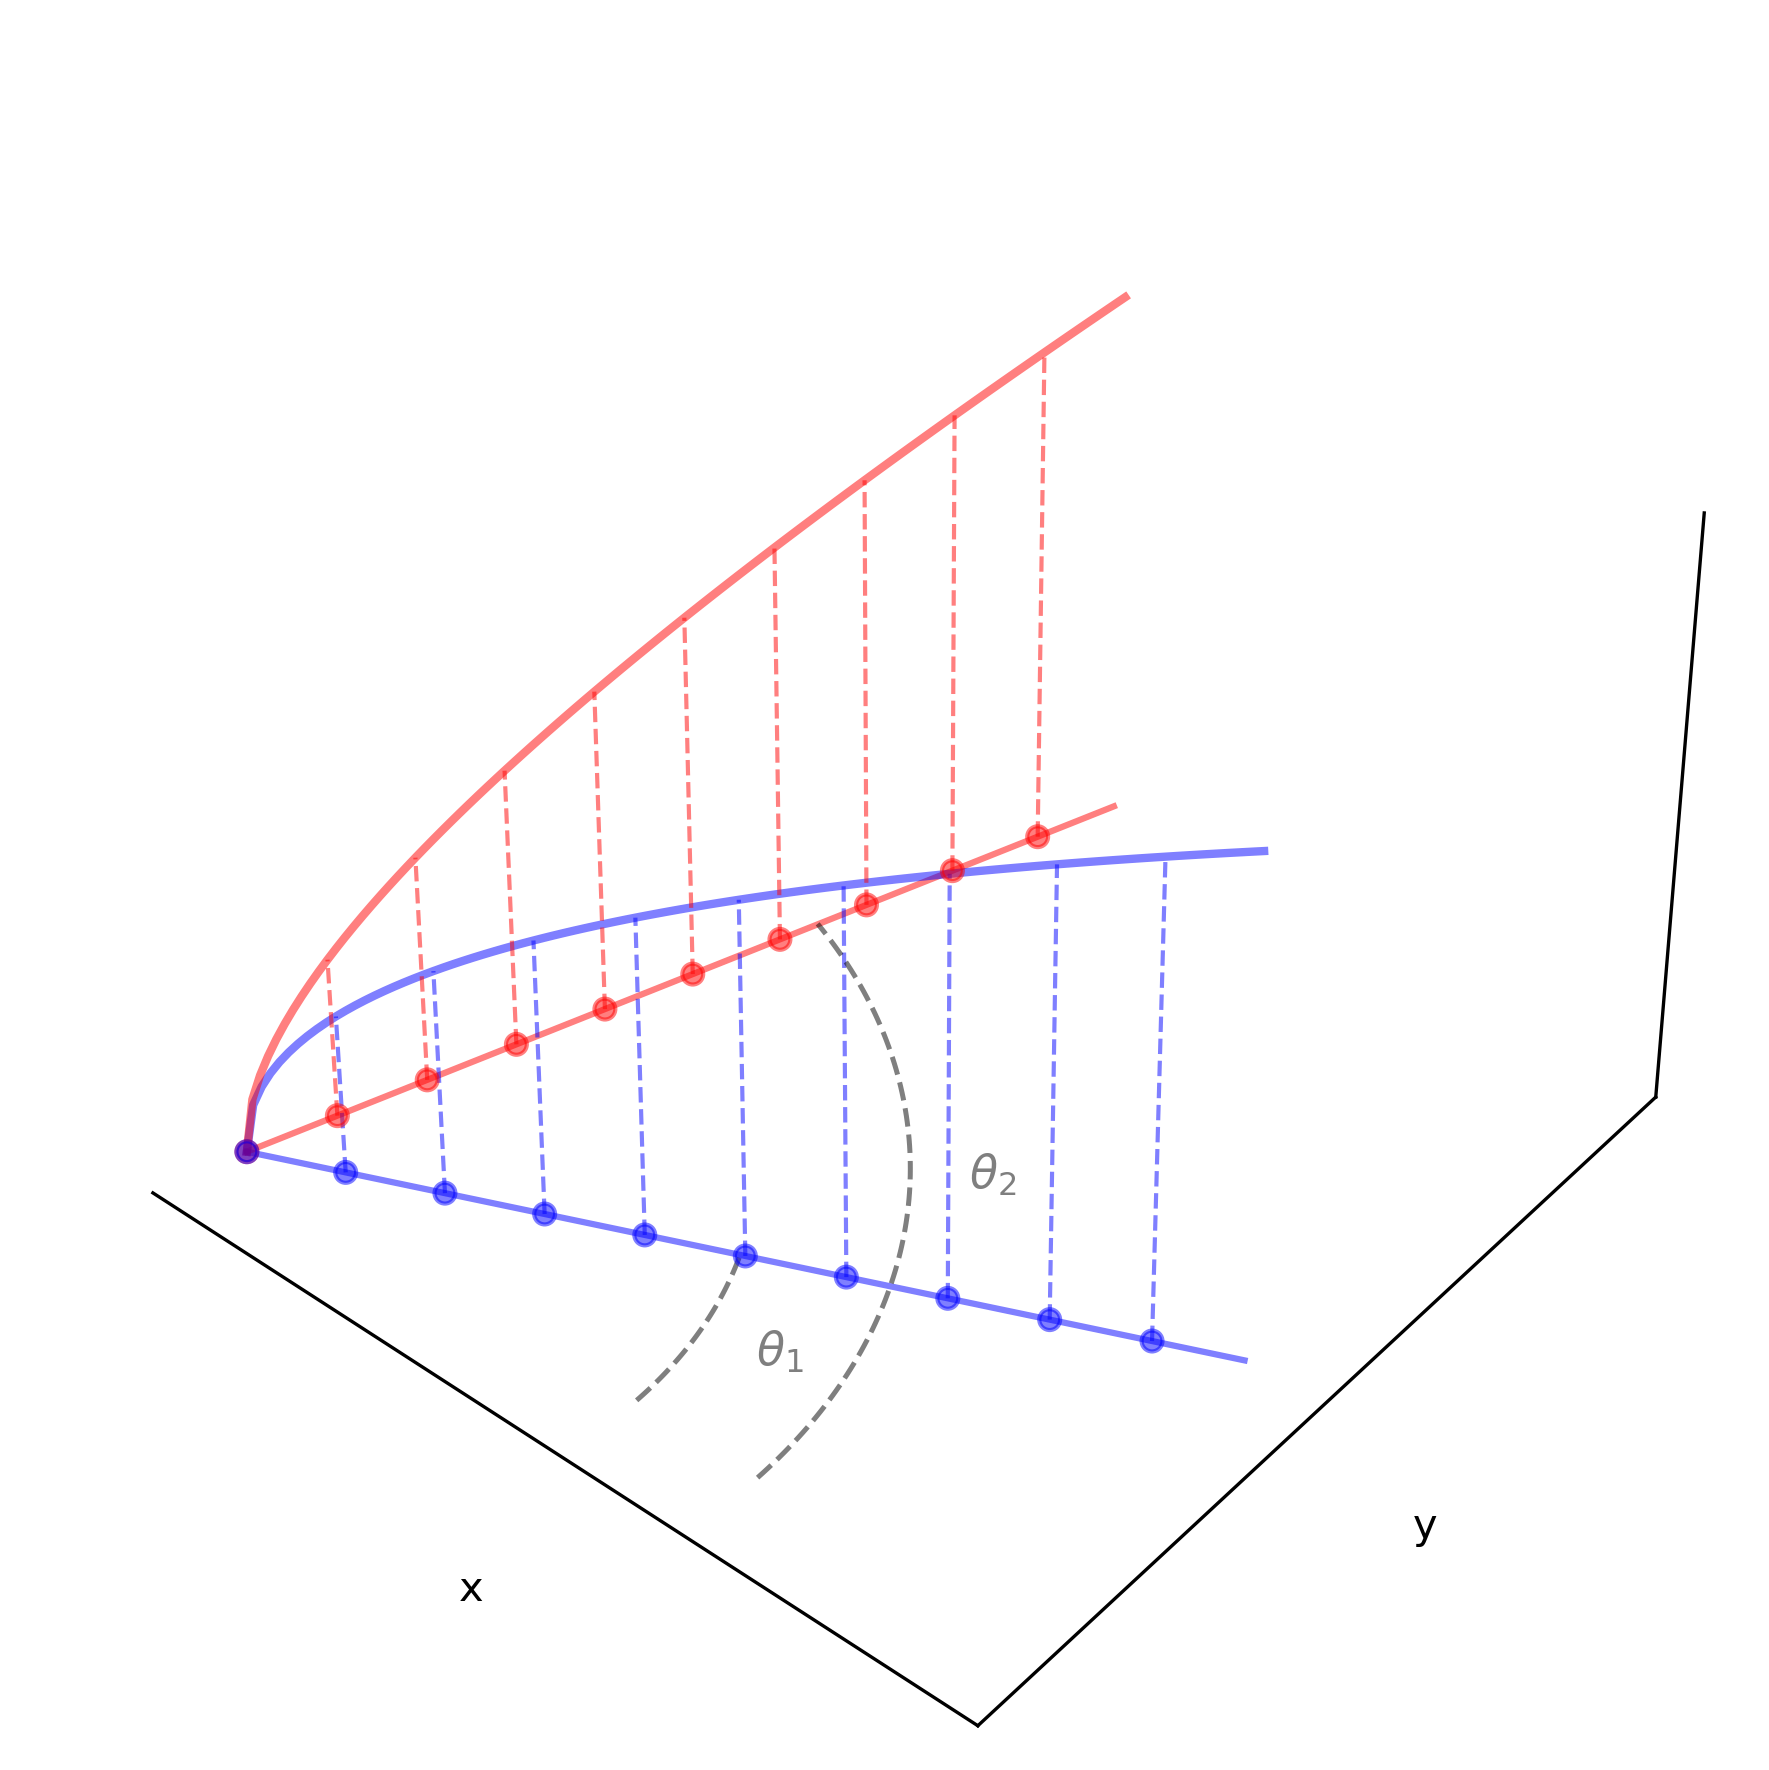
\includegraphics[width=8cm]{figures/SW1.png}};
\end{scope}

%%%%%%%%%%%%%%%%%%%%%%%%%%%%%%%%%%%%%%%%%%%%%
% Bottom-left: histogram (from ICDF samples)
%%%%%%%%%%%%%%%%%%%%%%%%%%%%%%%%%%%%%%%%%%%%%
\begin{scope}[shift={(-2.9,-3)}] % move/scale/rotate the whole panel here
  \node[anchor=south west, inner sep=0, scale=0.7] (img2) at (0,0)     {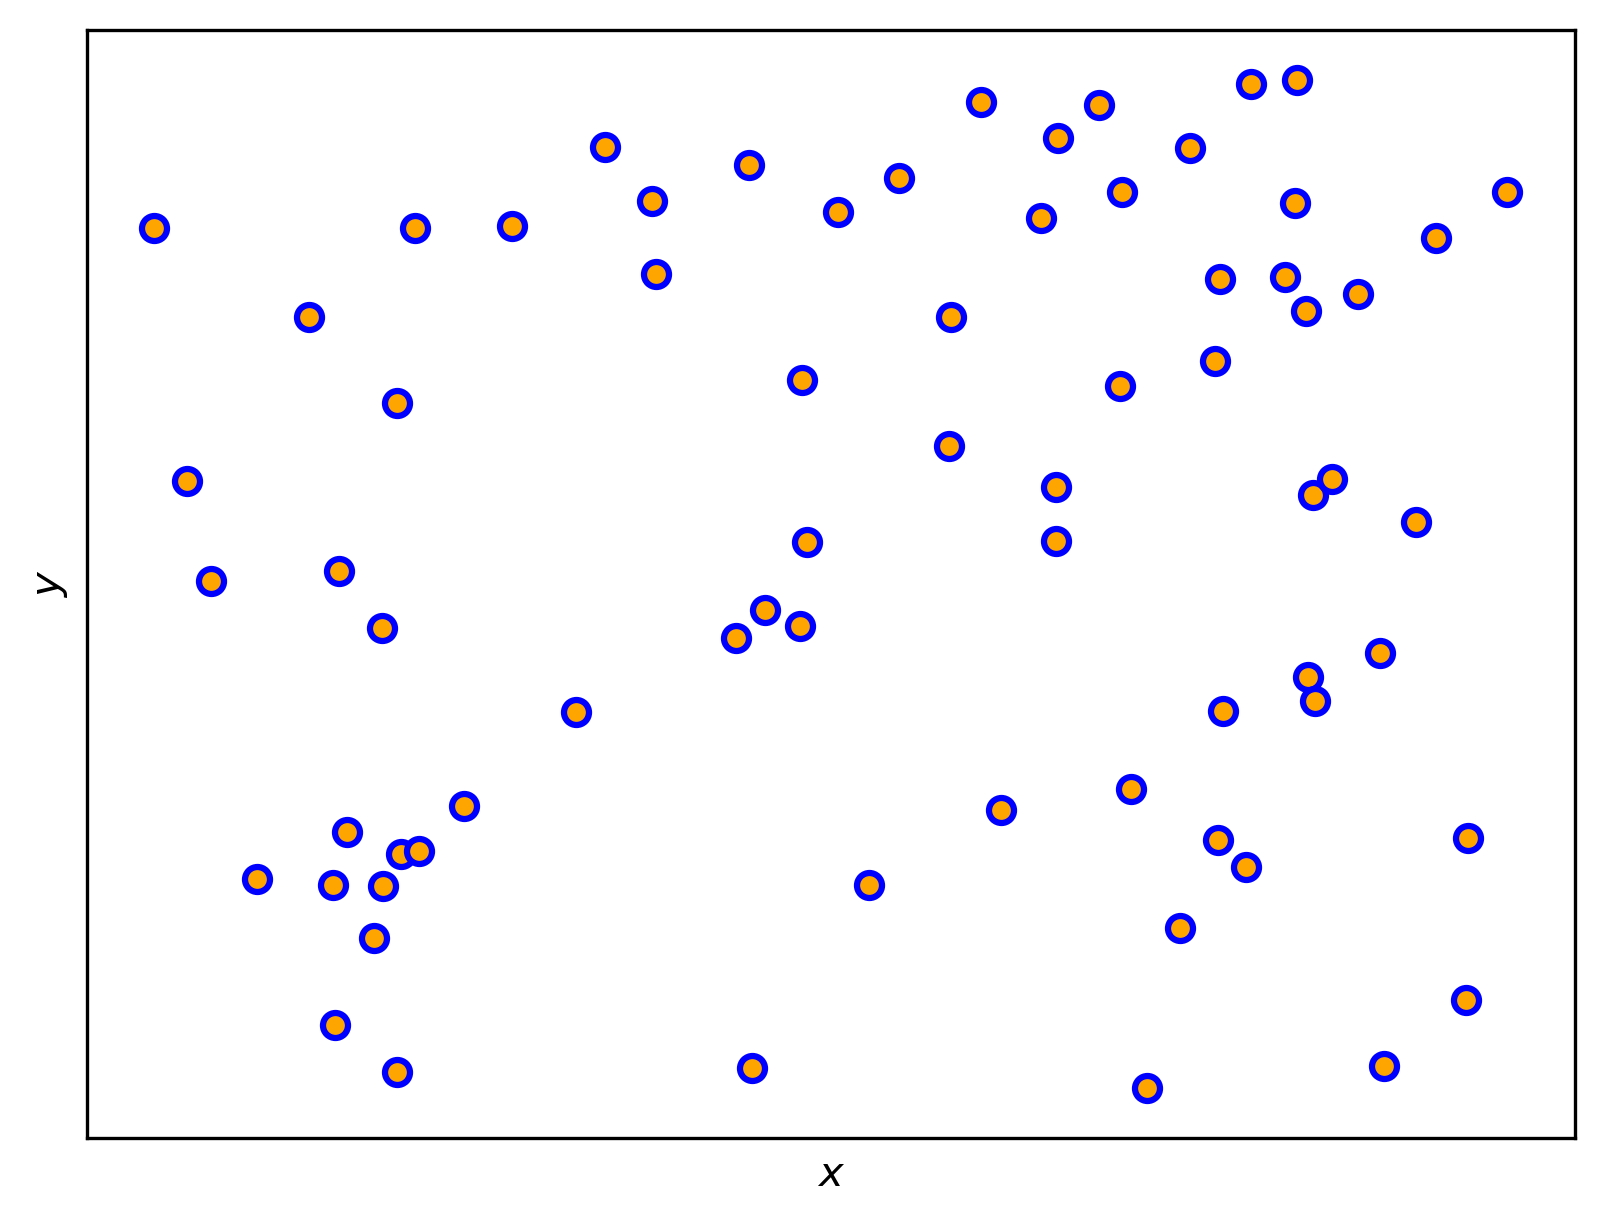
\includegraphics[width=8cm]{figures/particles1.png}};
\end{scope}

%%%%%%%%%%%%%%%%%%%%%%%%%%%%%%%%%%%%%%%%%%%%%
% Bottom-right: histogram after timestepper
%%%%%%%%%%%%%%%%%%%%%%%%%%%%%%%%%%%%%%%%%%%%%
\begin{scope}[shift={(7.5,-3)}] % move/scale/rotate the whole panel here
  \node[anchor=south west, inner sep=0, scale=0.68] (img3) at (0.0,0)     {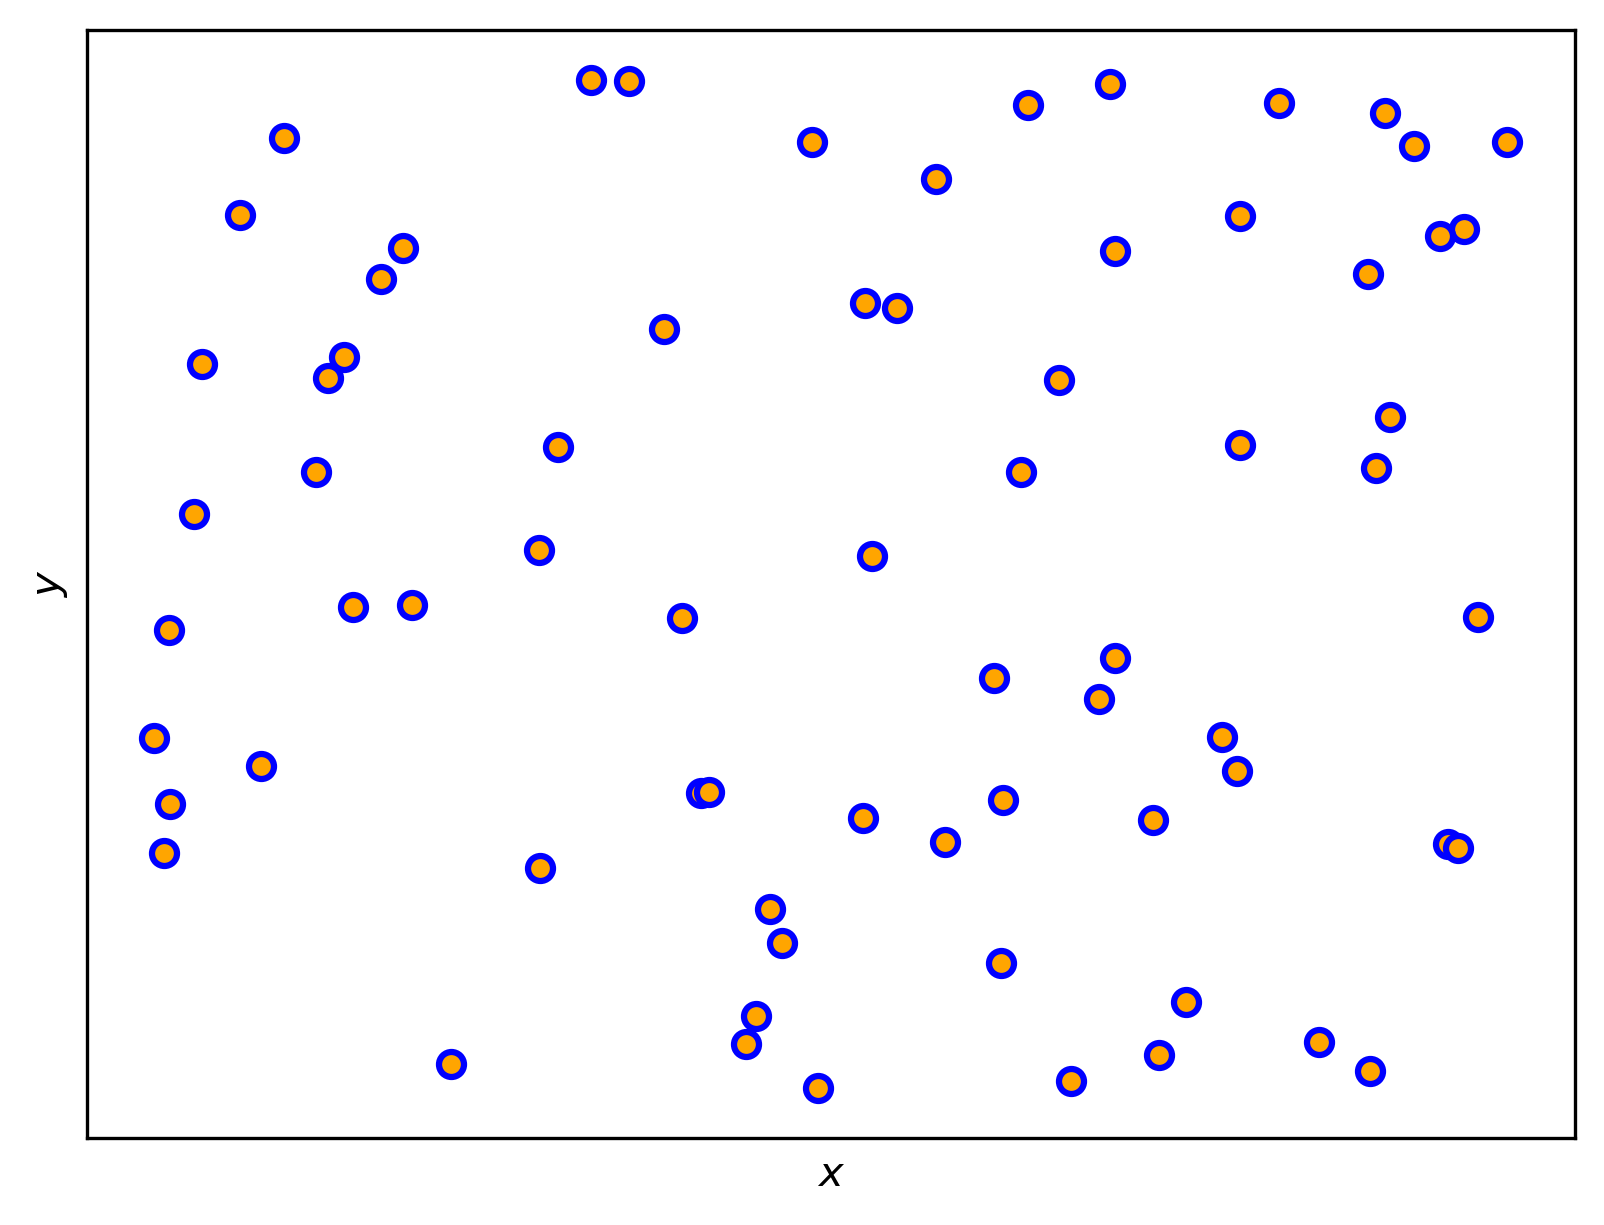
\includegraphics[width=8cm]{figures/particles2.png}};
\end{scope}

%%%%%%%%%%%%%%%%%%%%%%%%%%%%%%%%%%%%%
% Upper-right: slightly different ICDF
%%%%%%%%%%%%%%%%%%%%%%%%%%%%%%%%%%%%%
\begin{scope}[shift={(7.5,5)}]
    \node[anchor=south west, inner sep=0, scale=0.7] (img4) at (0,0)     {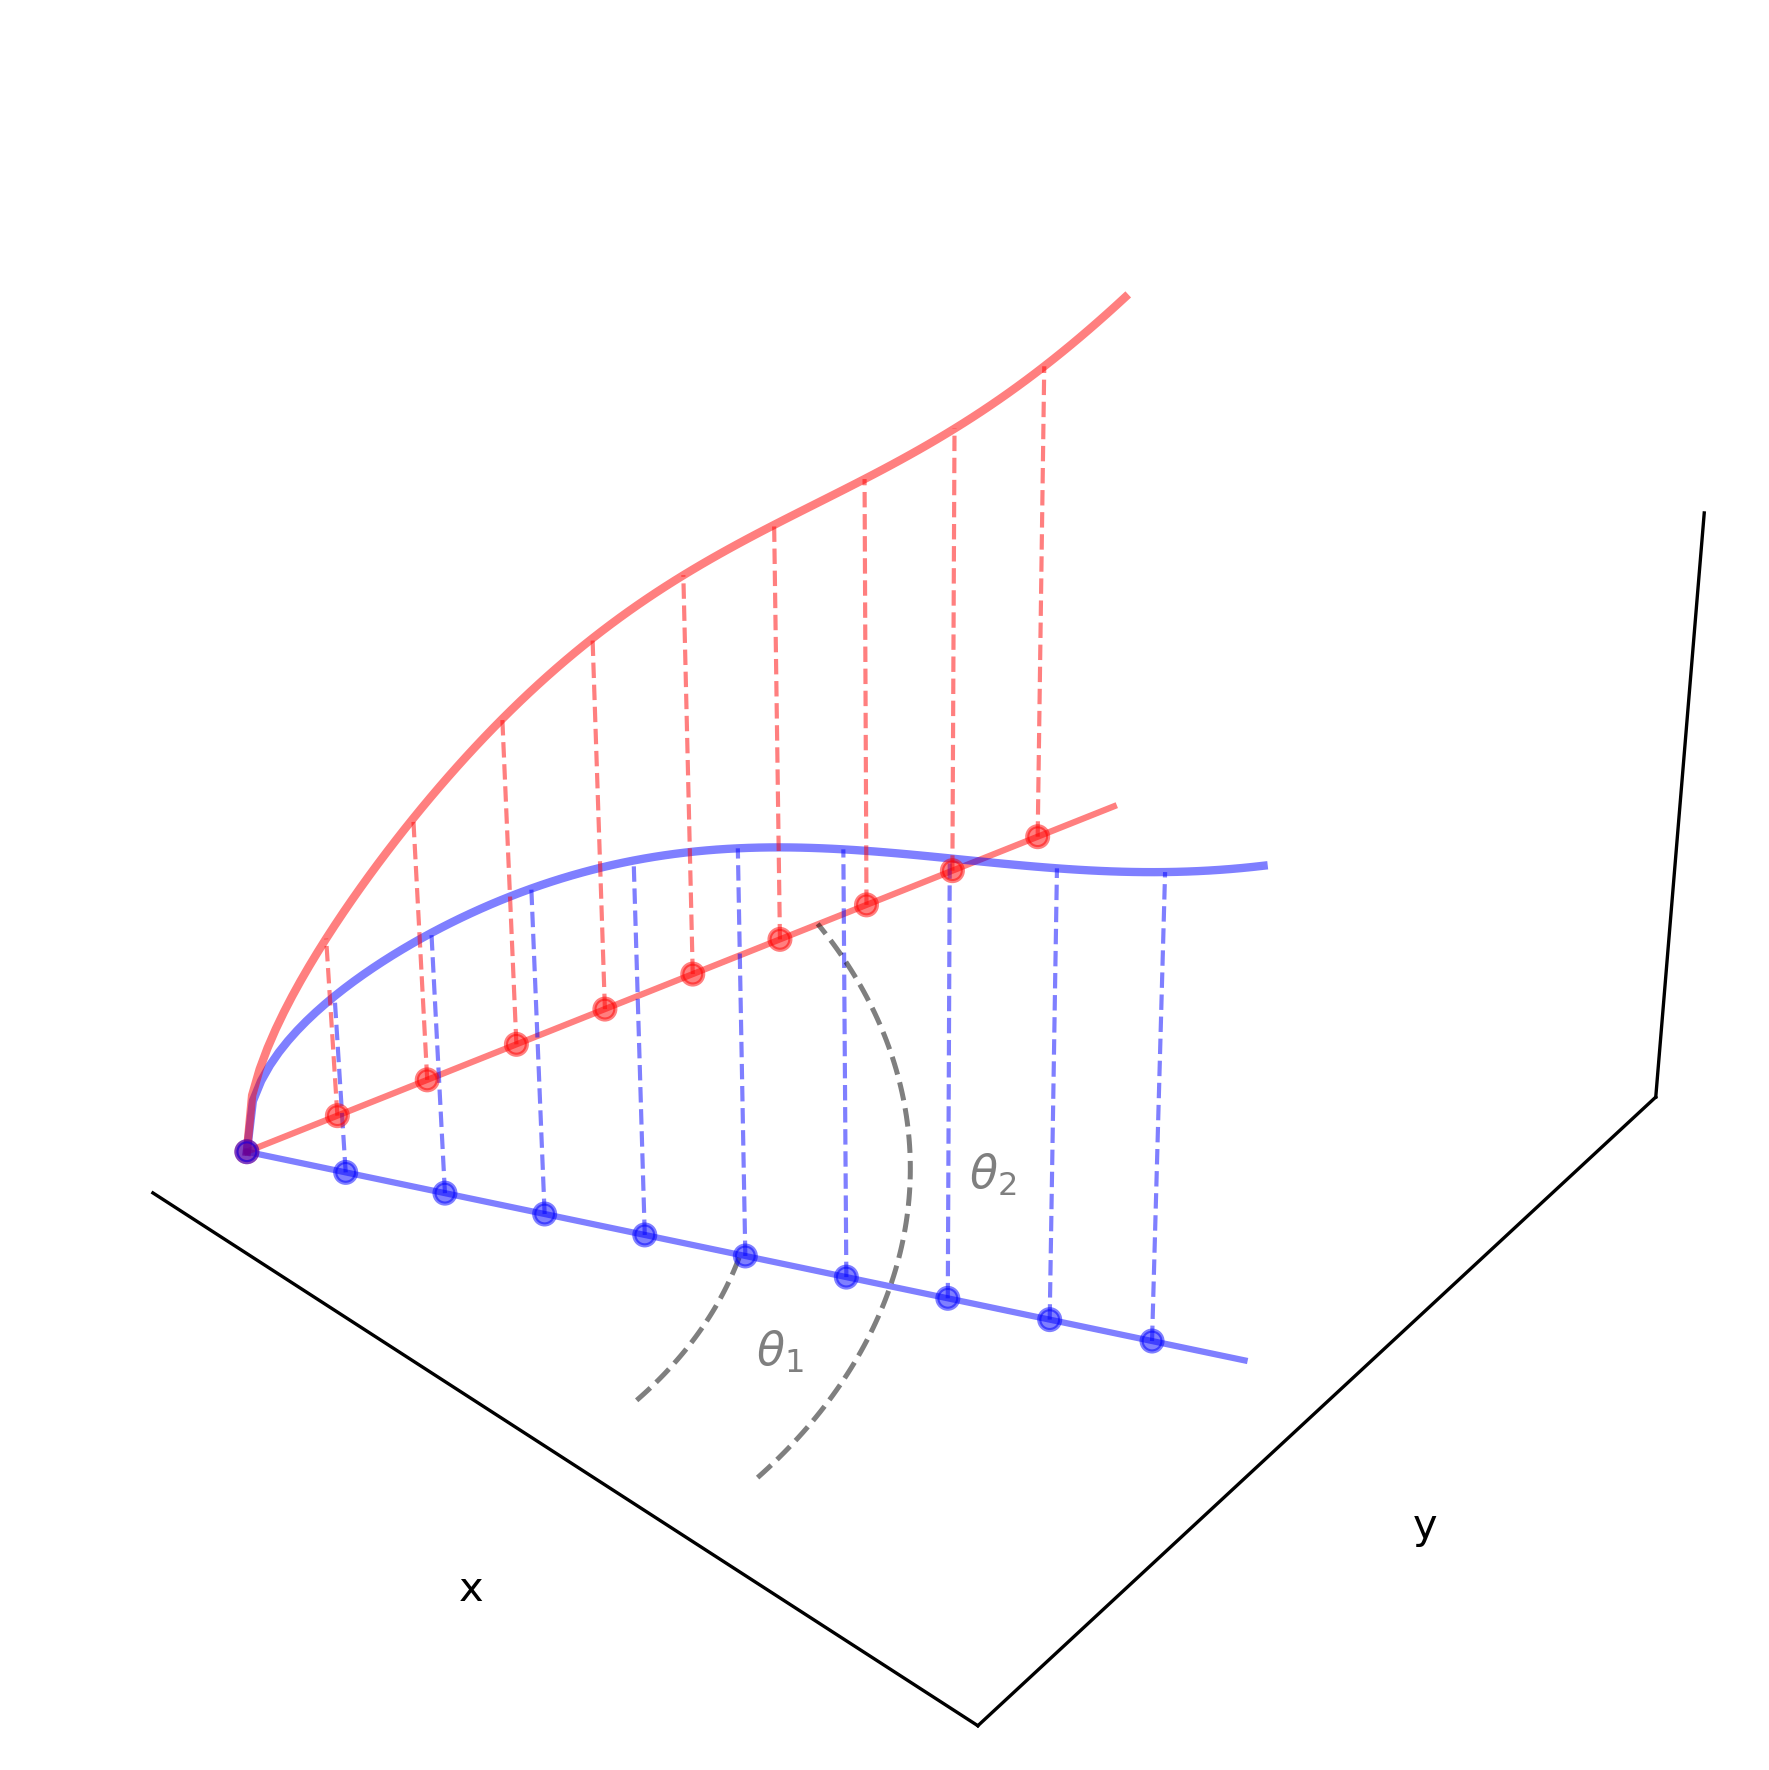
\includegraphics[width=8cm]{figures/SW2.png}};
\end{scope}

%%%%%%%%%%%%%%%%%%%%%%%%%%%%
% Arrows + labels
%%%%%%%%%%%%%%%%%%%%%%%%%%%%
\draw[arr, dashed] (3.7,7) -- (6.7,7);
\node[] at (5.1, 7.5) {Effective CDF Timestepper};
\draw[arr] (img1) -- (img2);
\node[align=center] at (2.2,3.2)
  {Sampling Directional \\ CDFs $F_t(x|\theta)$};
\draw[arr] (3.7,-0.5) -- (6.7,-0.5);
\node[] at (5.1, 0) {Particle Timestepper};
\draw[arr] (img3) -- (img4);
\node[align=center] at (12.2,3) {CDF by Counting \\ Particles below $x$ and $y$};

\end{tikzpicture}
\end{document}